%%% Template originaly created by Karol Kozioł (mail@karol-koziol.net) and modified for ShareLaTeX use

\documentclass[a4paper,11pt]{article}

\usepackage[T1]{fontenc}
\usepackage[utf8]{inputenc}
\usepackage{graphicx}
\usepackage{xcolor}
\usepackage{mathrsfs,amsmath} 
\usepackage{mathtools}
\usepackage{esint}
\usepackage{tgtermes}
\usepackage{physics}

\usepackage[
pdftitle={Phys 595 Assignment}, 
pdfauthor={Kenny Van, University of Alberta},
colorlinks=true,linkcolor=blue,urlcolor=blue,citecolor=blue,bookmarks=true,
bookmarksopenlevel=2]{hyperref}
\usepackage{amsmath,amssymb,amsthm,textcomp}
\usepackage{enumerate}
\usepackage{multicol}
\usepackage{tikz}

\usepackage{geometry}
\geometry{total={210mm,297mm},
left=25mm,right=25mm,%
bindingoffset=0mm, top=20mm,bottom=20mm}

\graphicspath{{./Images/}}

\linespread{1.3}

\newcommand{\linia}{\rule{\linewidth}{0.5pt}}

% custom theorems if needed
\newtheoremstyle{mytheor}
    {1ex}{1ex}{\normalfont}{0pt}{\scshape}{.}{1ex}
    {{\thmname{#1 }}{\thmnumber{#2}}{\thmnote{ (#3)}}}

\theoremstyle{mytheor}
\newtheorem{defi}{Definition}


% my own titles
\makeatletter
\renewcommand{\maketitle}{
\begin{center}
\vspace{2ex}
{\huge \textsc{\@title}}
\vspace{1ex}
\\
\linia\\
\@author \hfill \@date
\vspace{4ex}
\end{center}
}
\makeatother
%%%

% custom footers and headers
\usepackage{fancyhdr,lastpage}
\pagestyle{fancy}
\lhead{}
\chead{}
\rhead{}
\lfoot{Assignment 3}
\cfoot{}
\rfoot{Page \thepage\ /\ \pageref*{LastPage}}
\renewcommand{\headrulewidth}{0pt}
\renewcommand{\footrulewidth}{0pt}
%

%%%----------%%%----------%%%----------%%%----------%%%
\begin{document}

\title{Phys 595 - Astrophysical Fluids 3}
\author{Kenny Van}
\date{November 23, 2017}


\maketitle
\section*{Question 5}

Throughout the following question we will be solving the 1-d linear advection equation using a variety of discretization methods. For all cases the methods will be done in a domain of $[0,1]$ with velocity $ u = 1$ and periodic boundary conditions. The initial distribution will be a top-hat distribution given by:

\[
    a= 
\begin{cases}
    1, & \text{if } 0.4 \leq x \leq 0.6\\
    0, & \text{otherwise}
\end{cases}
\]

The period of simulation is given as $T = 1/u$ and we will test periods of $0.1$ and $1$. We will also test a variety of CFL numbers $C = 0.1, 0.33(3), 0.7$ and resolutions $\Delta x = 0.05, 0.033(3), 0.01$. It is important to note that $C \equiv \frac{u \Delta t}{\Delta x}$ we can see that timestep is calculated as $\Delta t = \frac{C \Delta x}{u}$. 

\subsection*{Upwind method}
\label{sec:Q5a}

Using upwind discretization we can solve the 1-d linear advection equation using an equation of the form:

\begin{equation}
    \frac{a_i^{n+1} - a_i^n}{\Delta t} = -u \frac{a_i^{n} - a_{i-1}^n}{\Delta x}
\label{eq:upwind}
\end{equation}

We can rearrange this equation to be in the form:

\begin{equation}
\begin{split}
    a_i^{n+1} & = \frac{-u \Delta t}{\Delta x} (a_i^{n} - a_{i-1}^n) + a_i^n \\
              & = - C (a_i^{n} - a_{i-1}^n) + a_i^n
\end{split}
\label{eq:upwind_a}
\end{equation}

Using this method we produce the figures \ref{fig:upwind_dx005}, \ref{fig:upwind_dx003} and \ref{fig:upwind_dx001}. From the results we can see that the solution is stable for all CFL numbers tested and the systems with higher resolution or lower $\Delta x$ retain the initial top-hat distribution better. The stability can be found through a fourier analysis of equation \ref{eq:upwind_a}. this will be done through a substitution of $a_j^n = A^n e^{ij \theta}$. Due to indexing from above we will replace our time index $i$ with $j$ and instead use $i$ to represent imaginary values.  The stability of the system is shown through:

\begin{equation}
\begin{split}
    A^{n+1} e^{ij\theta} &= -C (A^{n}e^{ij\theta} - A^n e^{i(j-1)\theta}) + A^n e^{ij\theta} \\
    \frac{A^{n+1}}{A^n} &= 1 - C(1 - e^{-i\theta}) \\
                        &= 1 - C + C(\cos\theta - i\sin\theta) \\
                        &= 1 - C(1 - \cos\theta) - iC\sin\theta \\
    \left|\frac{A^{n+1}}{A^n} \right| &= (1 - C(1 - \cos\theta))^2 - (iC\sin\theta)^2 \\
                        &= 1 - 2C(1-\cos\theta) + C^2(1 + \cos^2\theta - 2\cos\theta) + C^2\sin^2\theta \\
                        &= 1 - 2C + 2C\cos\theta + 2C^2 - 2C^2\cos^2\theta \\
                        &= 1 - 2C(1-C)(1-\cos\theta)
\end{split}
\end{equation}

Stability requires that $\left|\frac{A^{n+1}}{A^n} \right|^2 < 1$ so the criteria is:

\begin{equation}
\begin{split}
    |1 - 2C(1-C)(1-\cos\theta)| &\leq 1 \\
    -2C (1 - C)(1 - \cos\theta) &\leq 0 \\
    1 - C \geq 0 \\
    C \leq 1
\end{split}
\end{equation}

Diffusion can be shown by expanding equation \ref{eq:upwind}:

\begin{equation}
\begin{split}
     \frac{a_i^{n+1} - a_i^n}{\Delta t} &= -u \frac{a_i^{n} - a_{i-1}^n}{\Delta x} \\
                                        &= -u \left(\frac{a_{i+1}^n - a_{i-1}^n}{2\Delta x} - \Delta x \frac{(a_{i+1}^n - 2a_i^n + a_{i-1}^n)}{2\Delta x^2} \right) \\
                                        &= -u \frac{(a_{i+1}^n - a_{i-1}^n)}{2\Delta x} + \frac{u \Delta x}{2} \frac{(a_{i+1}^n - 2a_i^n + a_{i-1}^n)}{\Delta x^2} \\
                                        &= -u \frac{(a_{i+1}^n - a_{i-1}^n)}{2\Delta x} + D \frac{(a_{i+1}^n - 2a_i^n + a_{i-1}^n)}{\Delta x^2} 
\end{split}
\label{eq:upwind_diff}
\end{equation}

From equation \ref{eq:upwind_diff} we can see that the upwind method can be broken into two portions. The left portion is identical to the FTCS method, while the right portion is a diffusive term that prevents the upwind solution from being unstable. This numerical diffusion is given by $D = \frac{u \Delta x}{2}$. From this we see that with higher $\Delta x$ or lower resolution the diffusion is greater. The diffusion is more apparent when the system has taken more steps. This can be seen when the simulation period $T = 1.0$ as $a$ has decreased in comparison to $T = 0.1$. The initial distribution has diffused outwards more as the system has updated more times. In general it appears that a higher CFL number results in less diffusion. This is due to higher CFL numbers resulting in a larger $\Delta t$ when $u$ and $\Delta x$ are constant. With larger timesteps the system is updated fewer times resulting in less numeric diffusion.
\subsection*{FTCS Method}
\label{sec:Q5b}

Using FTCS discretization we can solve the 1-d linear advection equation using an equation of the form:

\begin{equation}
    \frac{a_i^{n+1} - a_i^n}{\Delta t} = -u \frac{a_{i+1}^{n} - a_{i-1}^n}{2 \Delta x}
\label{eq:FTCS}
\end{equation}

We can rearrange this equation to be in the form:

\begin{equation}
\begin{split}
    a_i^{n+1} & = \frac{-u \Delta t}{2 \Delta x} (a_{i+1}^{n} - a_{i-1}^n) + a_i^n \\
              & = - \frac{C}{2} (a_{i+1}^{n} - a_{i-1}^n) + a_i^n
\end{split}
\label{eq:FTCS_a}
\end{equation}

Using this method we produce the figures \ref{fig:FTCS_dx005}, \ref{fig:FTCS_dx003} and \ref{fig:FTCS_dx001}. As expected using the FTCS method the solution is unstable. This instability can be shown if we take the fourier transform of equation \ref{eq:FTCS_a}. 

\begin{equation}
\begin{split}
    A^{n+1}e^{ij\theta} &= - \frac{C}{2} (A^{n}e^{i(j+1)\theta} - A^{n}e^{i(j-1)\theta}) + A^{n}e^{i(j)\theta} \\
    A^{n+1} &= -\frac{C}{2} A^n(e^{i\theta} - e^{-i\theta}) + A^n \\
    A^{n+1} &= A^n(1 - iC \sin\theta) \\
    \left|\frac{A^{n+1}}{A^n}\right|^2 &= 1 + C^2 sin^2\theta
\end{split}
\label{eq:FTCS_fourier}
\end{equation}

We can see from equation \ref{eq:FTCS_fourier} that $\left|\frac{A^n+1}{A^n}\right|^2 > 1$. This means the FTCS is unstable for any CFL number. From equation \ref{eq:FTCS_fourier} we also see that the instability grows with $C$ which explains why larger CFL number peak at larger values. With a larger period these instabilities are more pronounced as the magnitude of the instability is proportional to $C^2$.
\subsection*{Implicit in Time Method}
\label{sec:Q5c}

The implicit-in-time discretization is given by the equation:

\begin{equation}
    \frac{a_i^{n+1}-a_i^n}{\Delta t} = -u\frac{a_i^{n+1}-a_{i-1}^{n+1}}{\Delta x}
\label{eq:IIT}
\end{equation}

Which similar to the previous methods can be rearranged:

\begin{equation}
\begin{split}
    a_i^{n+1} & = \frac{-u \Delta t}{\Delta x} (a_{i}^{n+1} - a_{i-1}^{n+1}) + a_i^n \\
              & = - C (a_{i}^{n+1} - a_{i-1}^{n+1}) + a_i^n \\
    a_i^n &= -C a_{i-1}^{n+1} + (1+C) a_{i}^{n+1}
\end{split}
\label{eq:IIT_a}
\end{equation}

Which when written in matrix form is generally given as:

\begin{equation}
\begin{pmatrix}
1+C &     &     &        &        &     & -C  \\
-C  & 1+C &     &        &        &     &     \\
    & -C  & 1+C &        &        &     &     \\
    &     & -C  & 1+C    &        &     &     \\
    &     &     & \ddots & \ddots &     &     \\
    &     &     &        & -C     & 1+C &     \\
    &     &     &        &        & -C  & 1+C \\
\end{pmatrix}
\begin{pmatrix}
u_1^{n+1}     \\
u_2^{n+1}     \\
u_3^{n+1}     \\
u_4^{n+1}     \\
\vdots        \\
u_{N-2}^{n+1} \\
u_{N-1}^{n+1} \\
\end{pmatrix}
=
\begin{pmatrix}
u_1^{n}     \\
u_2^{n}     \\
u_3^{n}     \\
u_4^{n}     \\
\vdots      \\
u_{N-2}^{n} \\
u_{N-1}^{n} \\
\end{pmatrix}
\end{equation}

To solve for $B$ in an equation of the form $AB = X$  we must take the inverse of $A$ and perform $A^{-1}AB = A^{-1}X$ which becomes $B = A^{-1}X$. We can find the inverse of our matrix using the Gauss-Jordan elimination Method. To do this we append an identity matrix to the matrix which we wish to invert. From here we use basic row operations to change our matrix $A$ into row-echelon form. This will also apply the operations to the identity matrix which once our matrix $A$ is in row-echelon form, the right hand matrix will be $A^{-1}$.

\begin{equation*}
\left(
\begin{array}{@{}ccccc|ccccc@{}}
1+C &        &        &     & -C  & 1 &   &        &   &   \\
-C  & 1+C    &        &     &     &   & 1 &        &   &   \\
    & \ddots & \ddots &     &     &   &   & \ddots &   &   \\
    &        & -C     & 1+C &     &   &   &        & 1 &   \\    
    &        &        & -C  & 1+C &   &   &        &   & 1 \\    
\end{array}
\right)
\end{equation*}

By doing this we can produce figures \ref{fig:IIT_dx005}, \ref{fig:IIT_dx003} and \ref{fig:IIT_dx001}. Similar to the upwind method, the implicit-in-time method produces a stable solution. Again if we perform a similar analysis as with the upwind method we can see that a numeric diffusion term is present. 

\begin{equation}
\begin{split}
     \frac{a_i^{n+1} - a_i^n}{\Delta t} &= -u \frac{a_i^{n+1} - a_{i-1}^{n+1}}{\Delta x} \\
                                        &= -u \left(\frac{a_{i+1}^{n+1} - a_{i-1}^{n+1}}{2\Delta x} - \Delta x \frac{(a_{i+1}^{n+1} - 2a_i^{n+1} + a_{i-1}^{n+1})}{2\Delta x^2} \right) \\
                                        &= -u \frac{(a_{i+1}^{n+1}- a_{i-1}^{n+1})}{2\Delta x} + \frac{u \Delta x}{2} \frac{(a_{i+1}^{n+1} - 2a_i^{n+1} + a_{i-1}^{n+1})}{\Delta x^2} \\
                                        &= -u \frac{(a_{i+1}^{n+1} - a_{i-1}^{n+1})}{2\Delta x} + D \frac{(a_{i+1}^{n+1} - 2a_i^{n+1} + a_{i-1}^{n+1})}{\Delta x^2} 
\end{split}
\label{eq:IIT_diff}
\end{equation}

The effect of the resolution is again apparent with lower resolution producing a more diffuse solution with the diffusion term being represented by $D = \frac{u\Delta x}{2}$. The key difference between the implicit-in-time solution and the upwind solution is that the CFL number has a smaller effect in the implicit-in-time method. While changes in the CFL number resulted in significant changes in $a$ for the upwind method, there is a much smaller difference in the implicit-in-time method. Another difference is that the higher CFL number produces smaller $a$ values in the implicit-in-time method instead of larger $a$ values in the upwind method.


\begin{figure}[h]
    \centering
    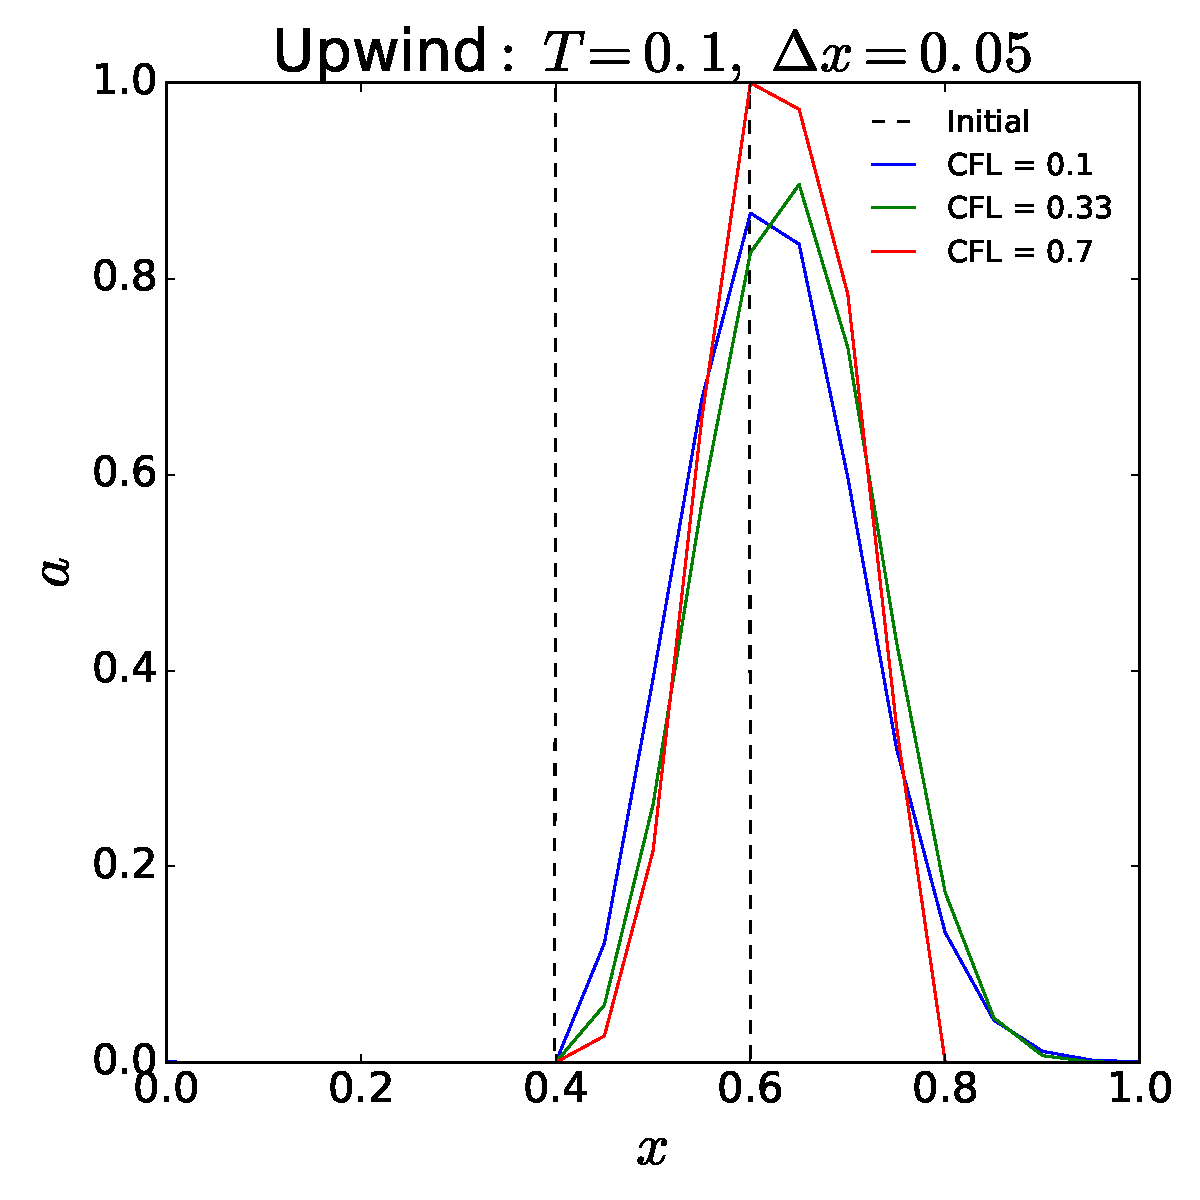
\includegraphics[width=0.45\columnwidth]{upwind_T01_dx005.pdf}
    \hspace{0.05pt}
    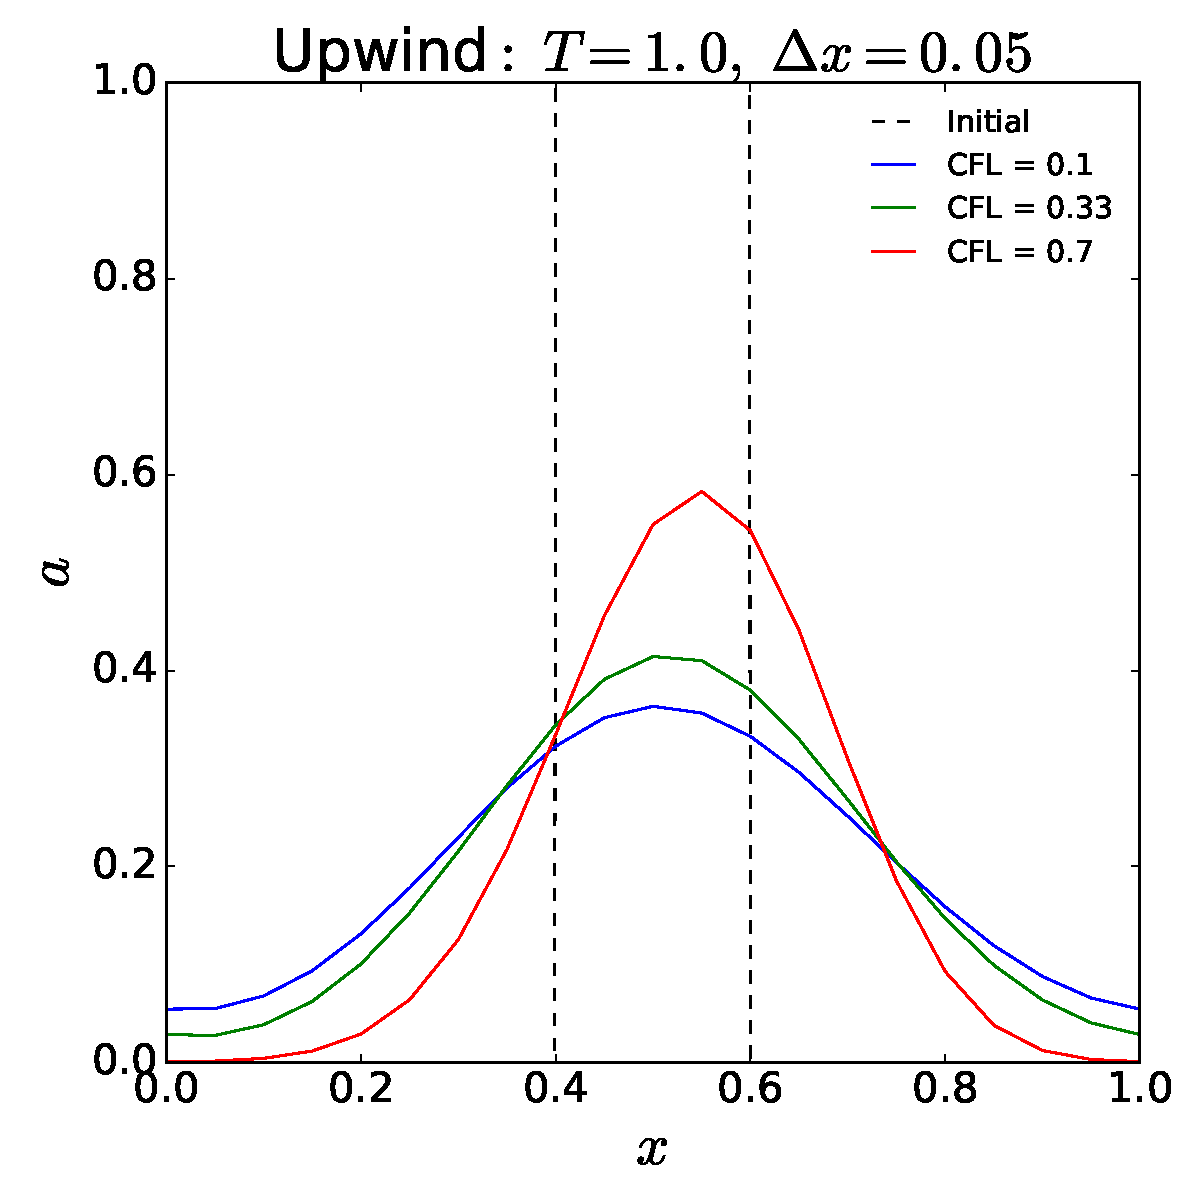
\includegraphics[width=0.45\columnwidth]{upwind_T10_dx005.pdf}
    \caption{The system after $T=0.1$ and $T=1.0$ with resolution $\Delta x=0.05$}
    \label{fig:upwind_dx005}
\end{figure}

\begin{figure}[h]
    \centering
    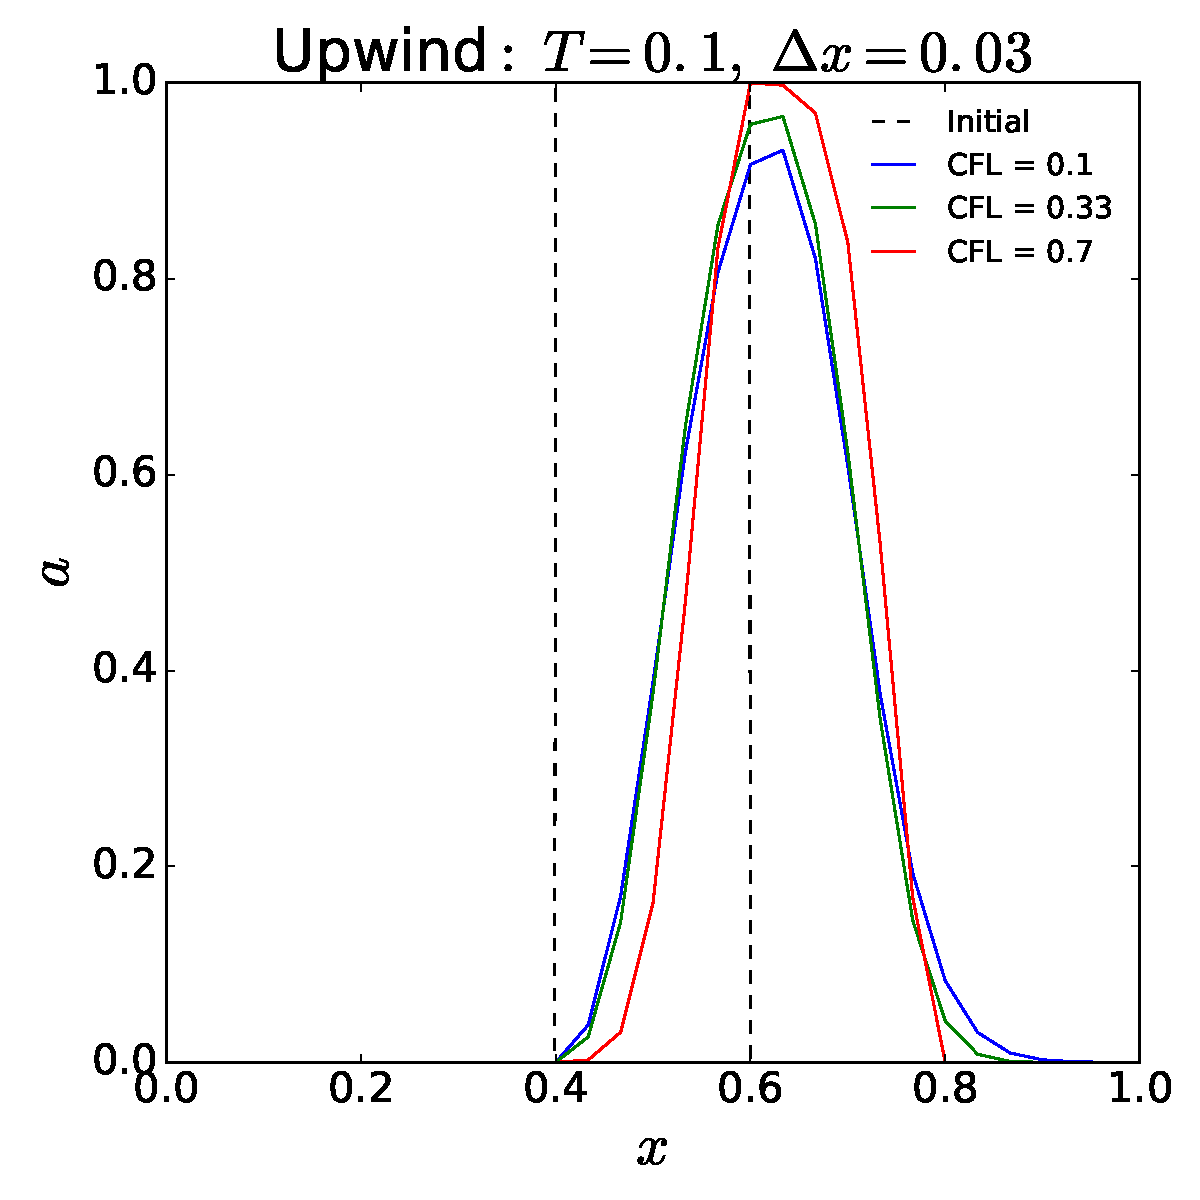
\includegraphics[width=0.45\columnwidth]{upwind_T01_dx003.pdf}
    \hspace{0.05pt}
    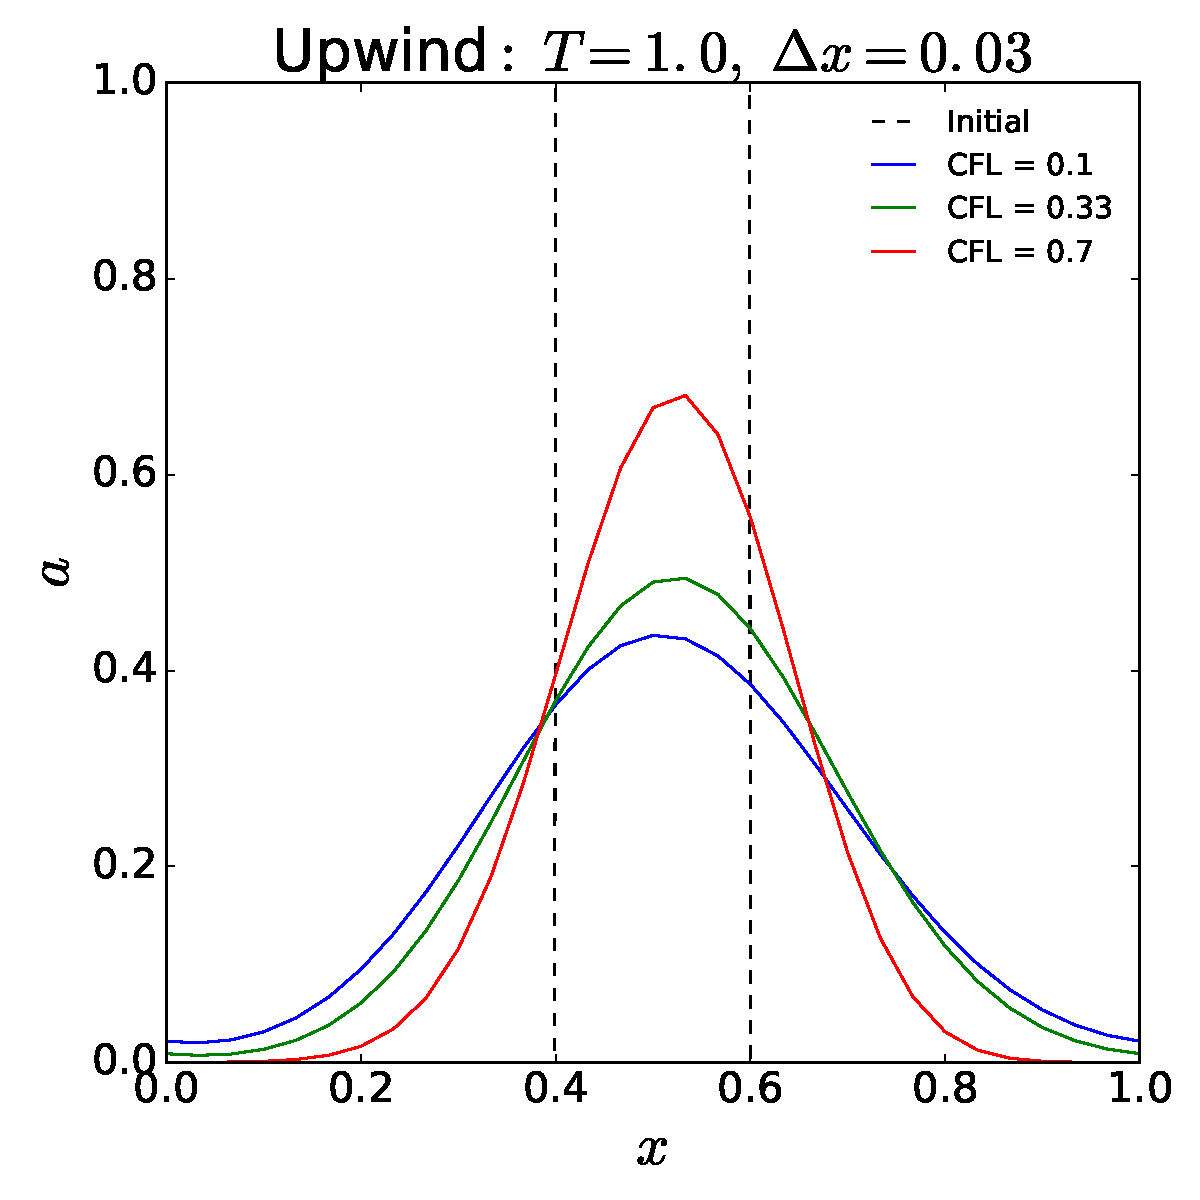
\includegraphics[width=0.45\columnwidth]{upwind_T10_dx003.pdf}
    \caption{The system after $T=0.1$ and $T=1.0$ with resolution $\Delta x=0.03$}
    \label{fig:upwind_dx003}
\end{figure}

\begin{figure}[h]
    \centering
    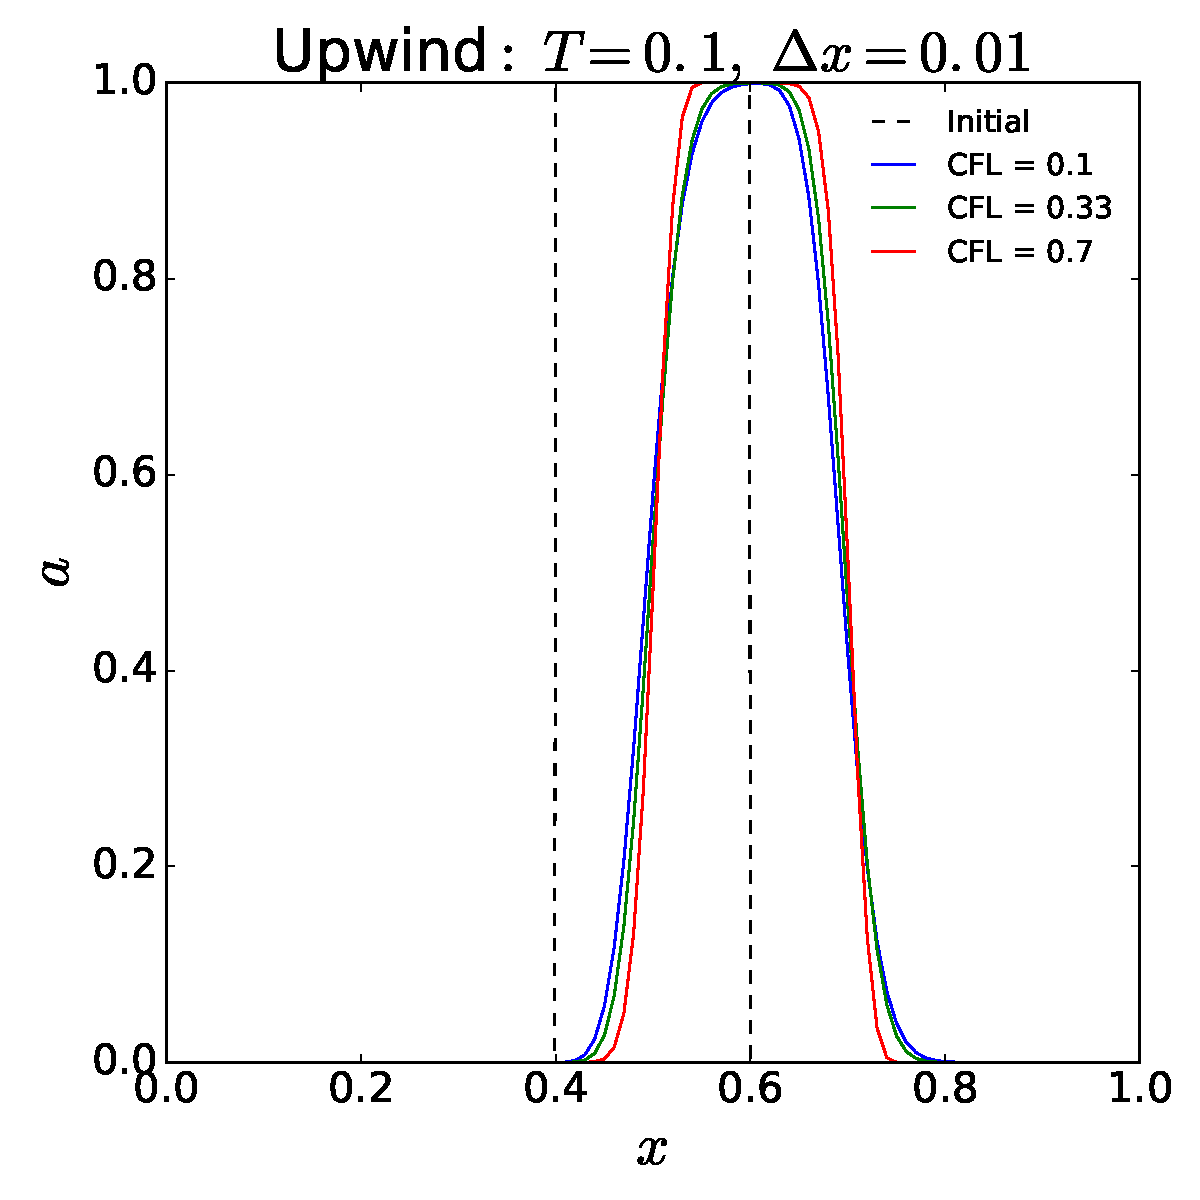
\includegraphics[width=0.45\columnwidth]{upwind_T01_dx001.pdf}
    \hspace{0.05pt}
    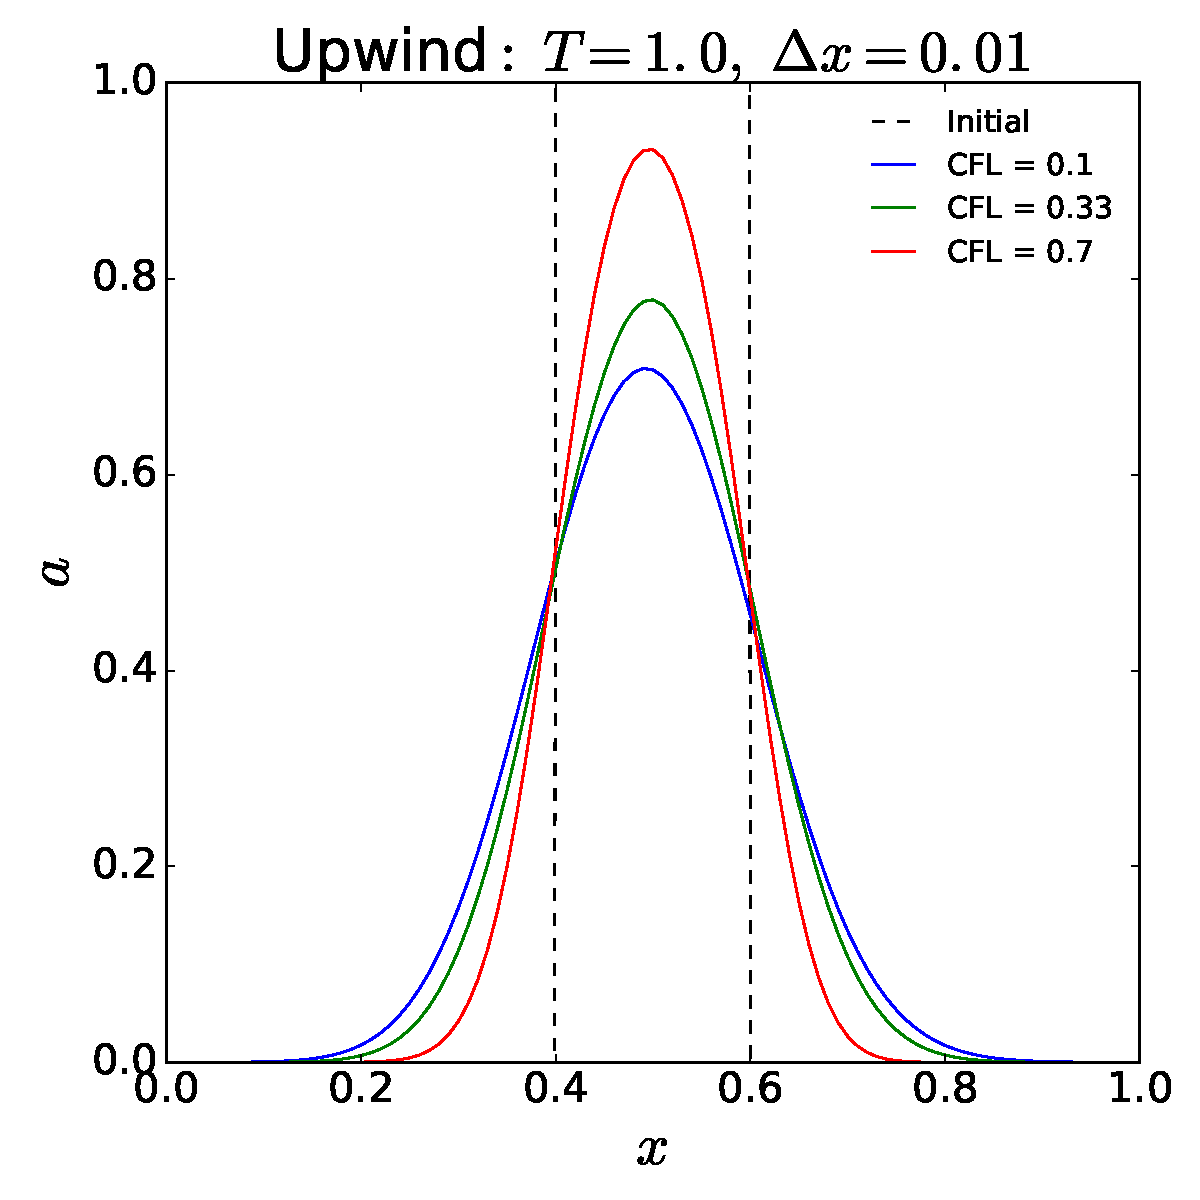
\includegraphics[width=0.45\columnwidth]{upwind_T10_dx001.pdf}
    \caption{The system after $T=0.1$ and $T=1.0$ with resolution $\Delta x=0.01$}
    \label{fig:upwind_dx001}
\end{figure}

\begin{figure}[h]
    \centering
    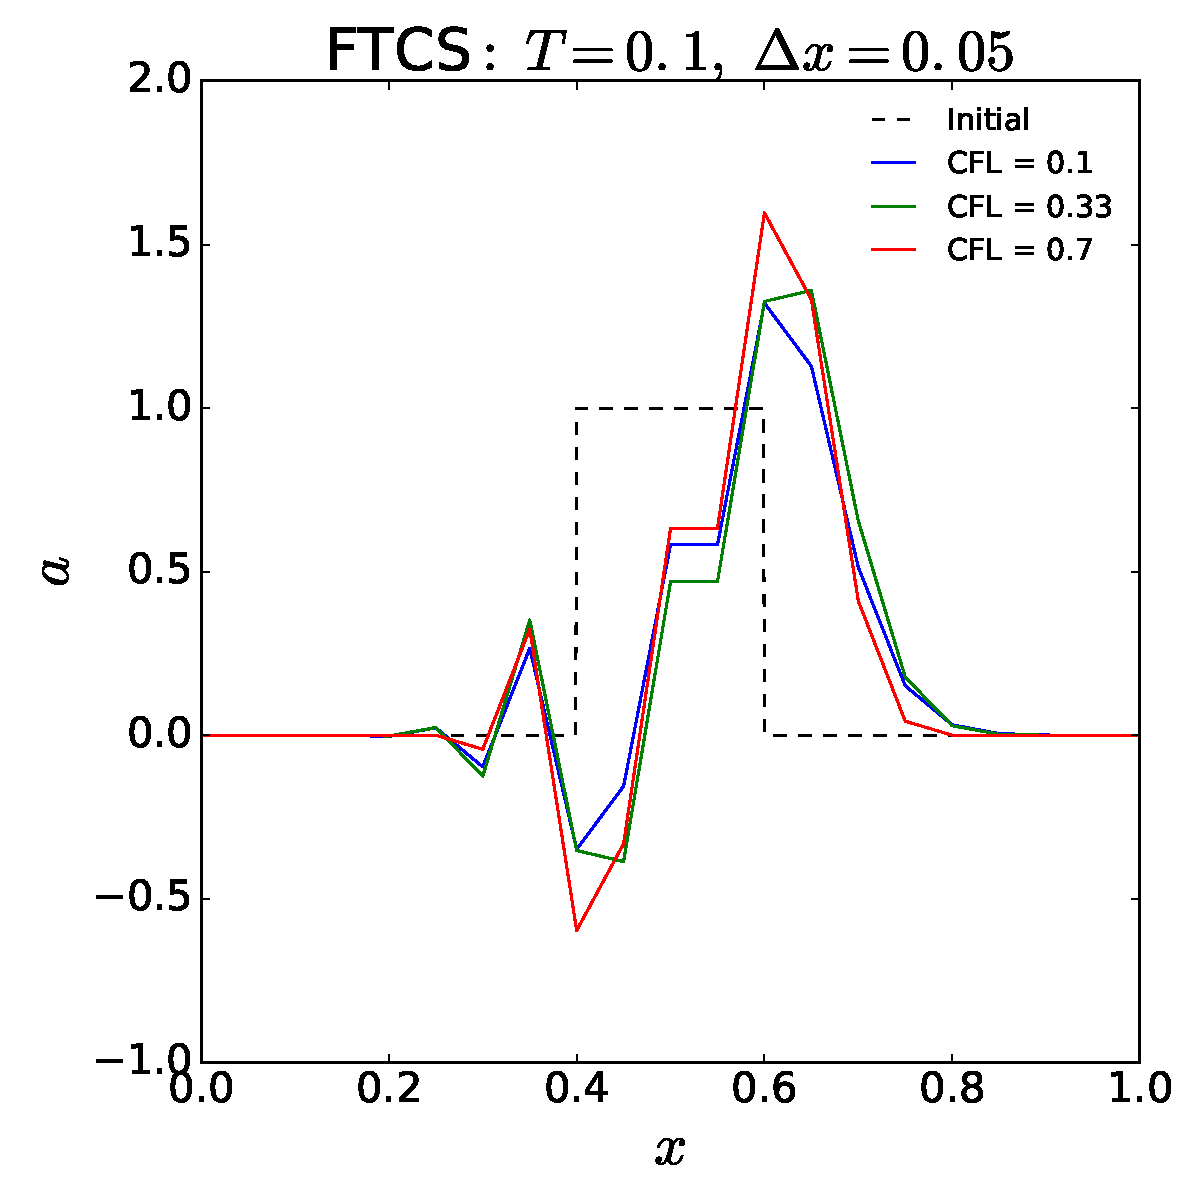
\includegraphics[width=0.45\columnwidth]{FTCS_T01_dx005.pdf}
    \hspace{0.05pt}
    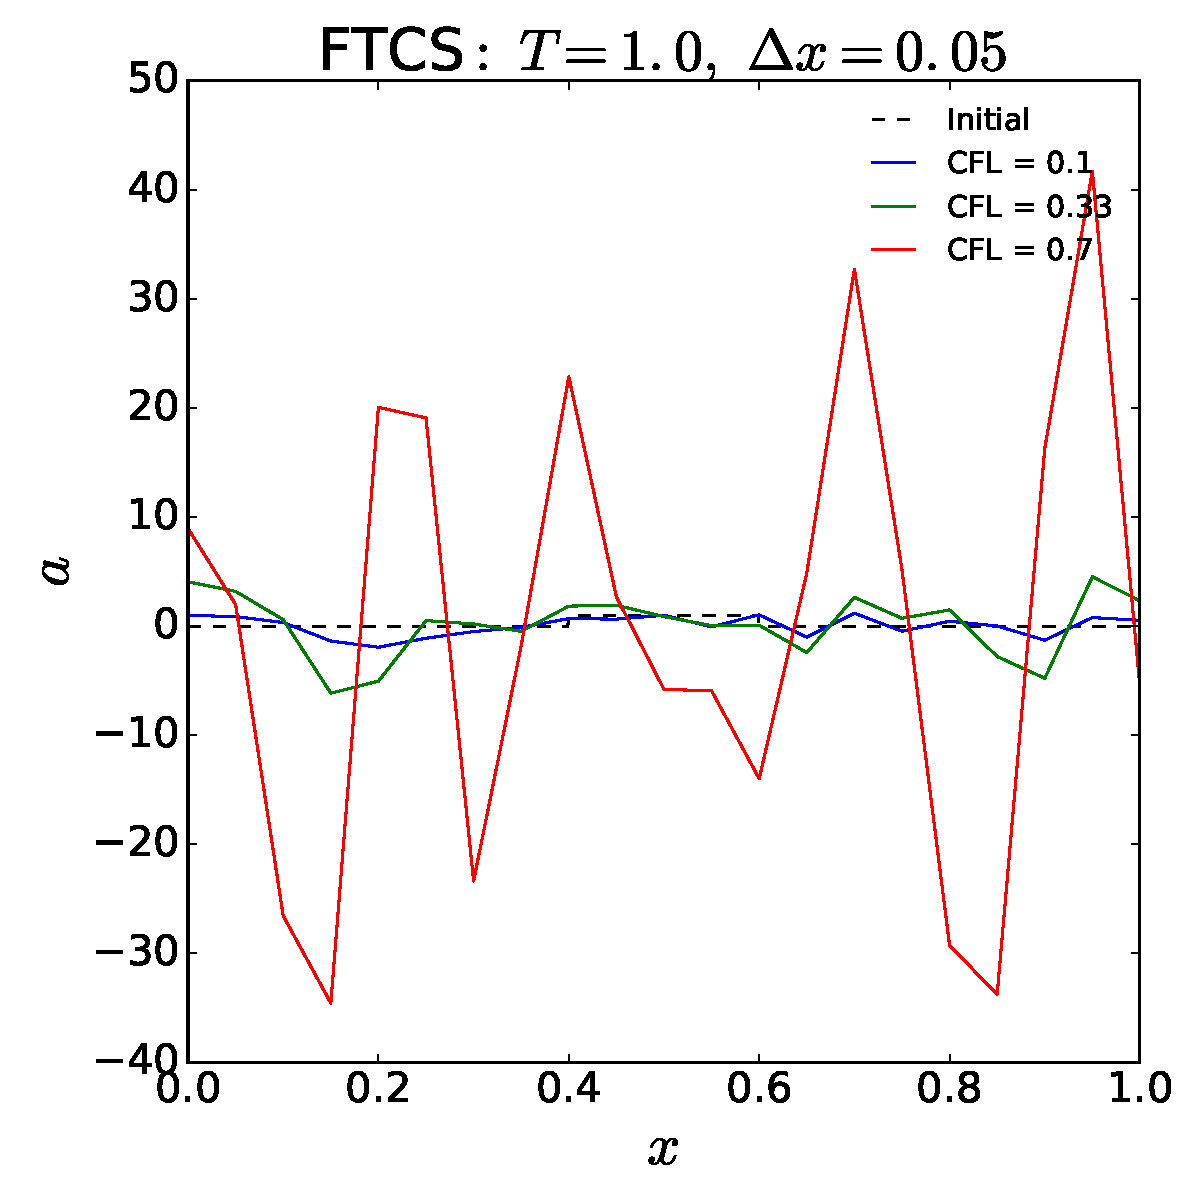
\includegraphics[width=0.45\columnwidth]{FTCS_T10_dx005.pdf}
    \caption{The system after $T=0.1$ and $T=1.0$ with resolution $\Delta x=0.05$}
    \label{fig:FTCS_dx005}
\end{figure}

\begin{figure}[h]
    \centering
    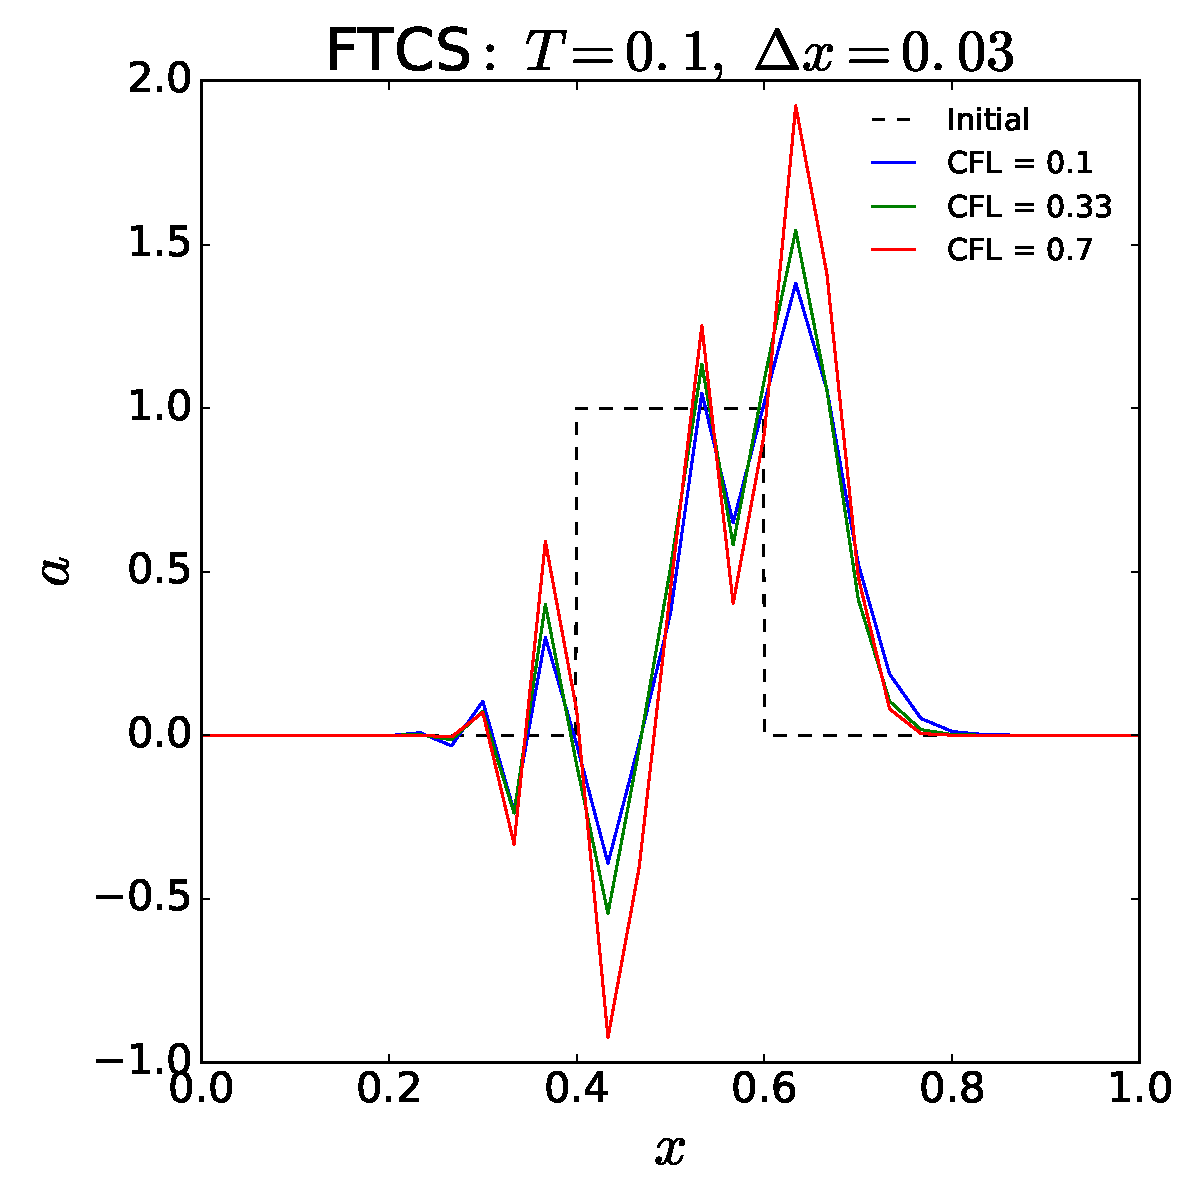
\includegraphics[width=0.45\columnwidth]{FTCS_T01_dx003.pdf}
    \hspace{0.05pt}
    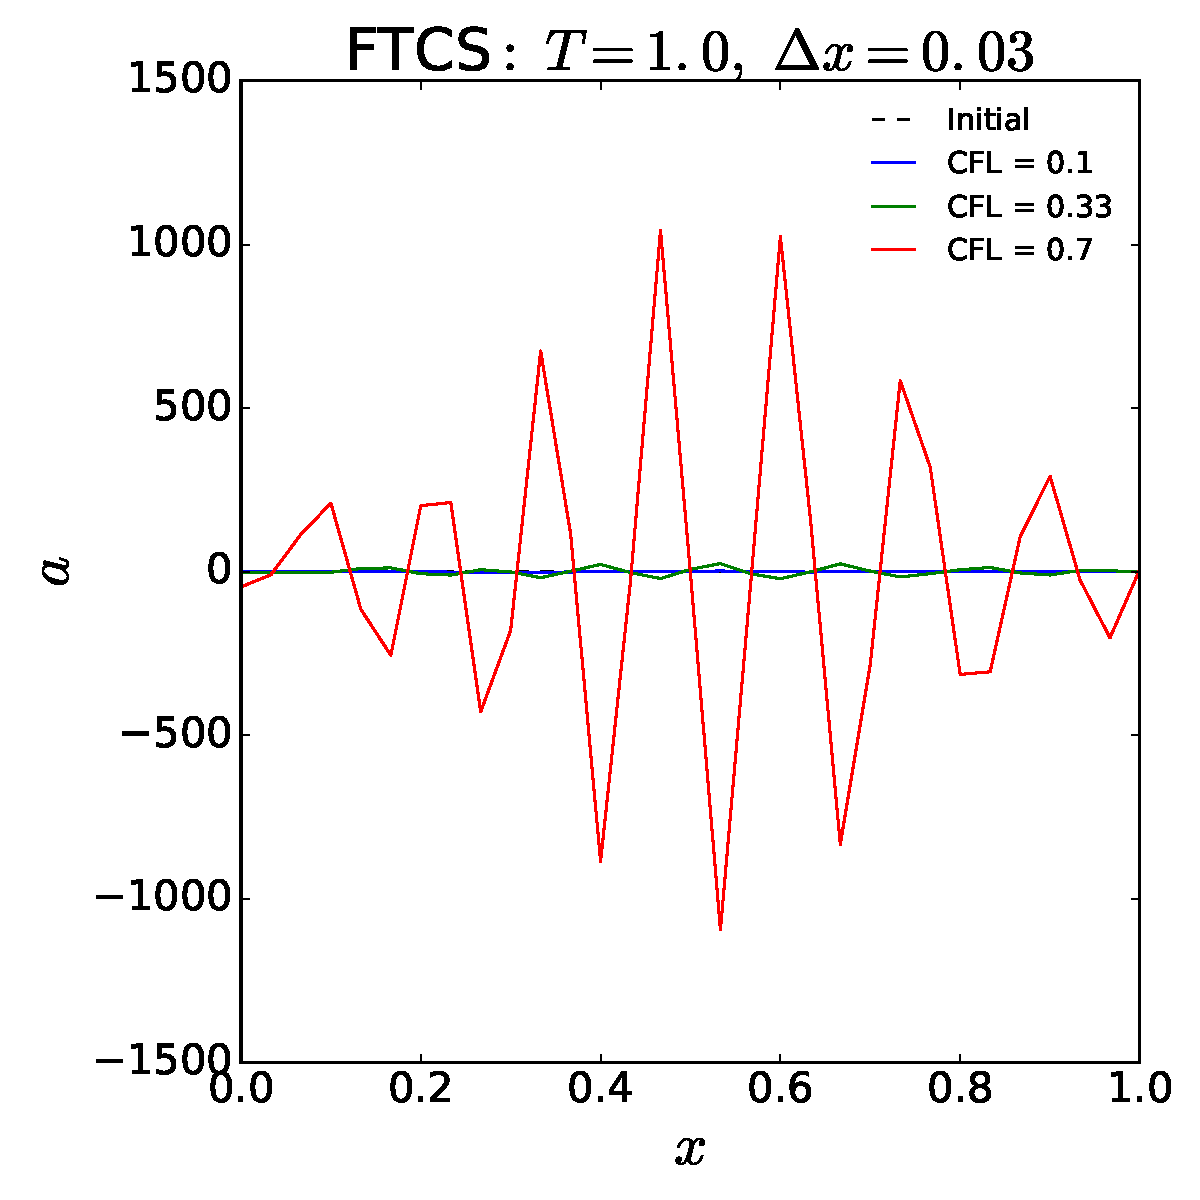
\includegraphics[width=0.45\columnwidth]{FTCS_T10_dx003.pdf}
    \caption{The system after $T=0.1$ and $T=1.0$ with resolution $\Delta x=0.03$}
    \label{fig:FTCS_dx003}
\end{figure}

\begin{figure}[h]
    \centering
    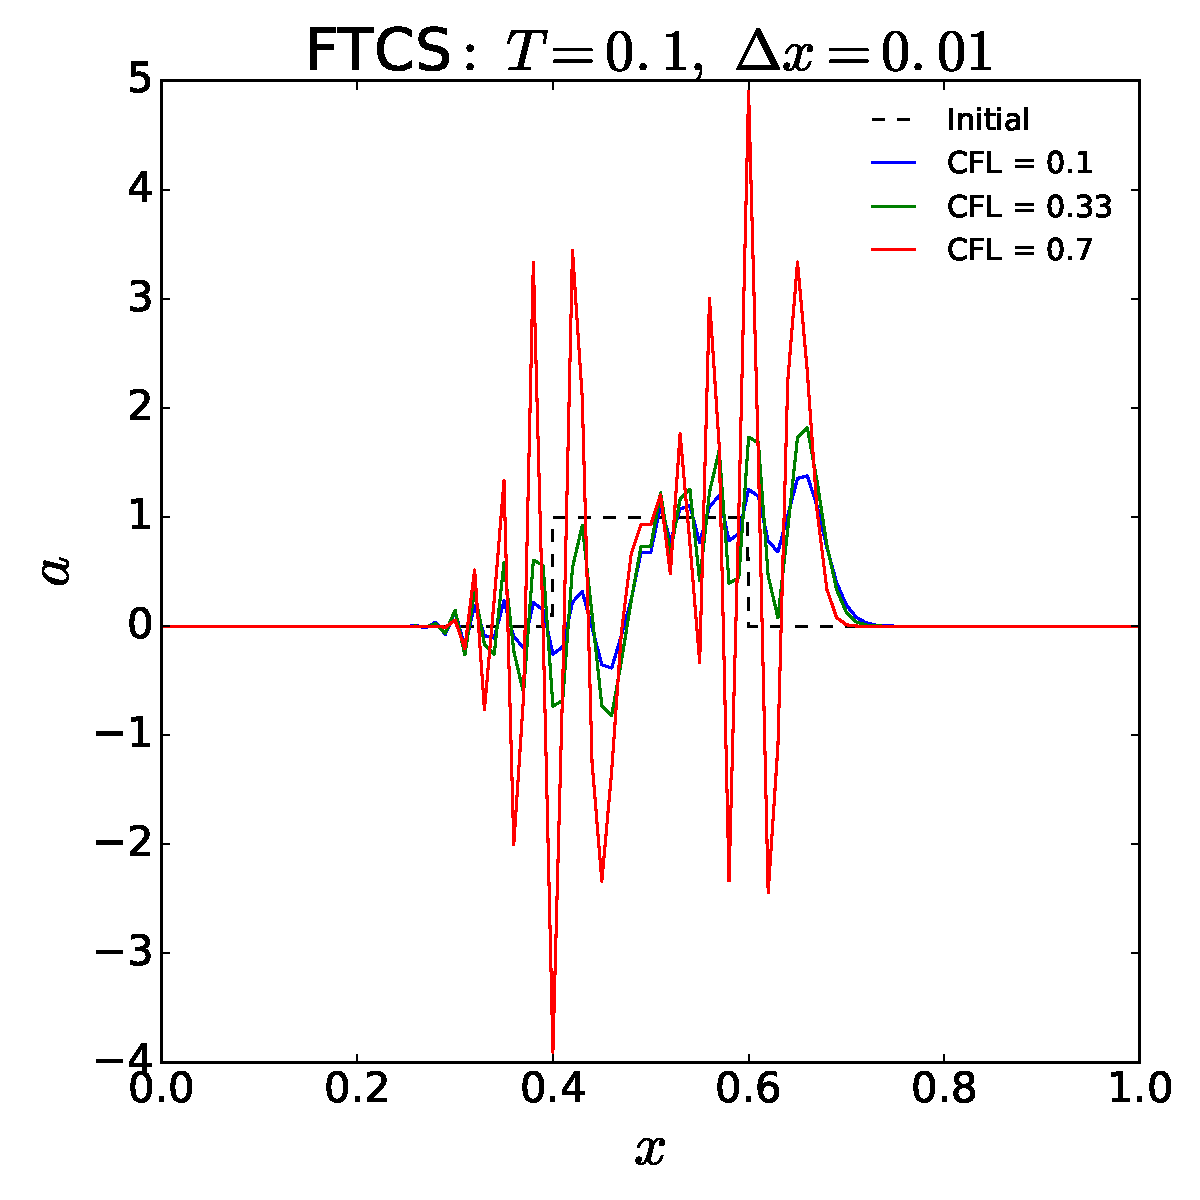
\includegraphics[width=0.45\columnwidth]{FTCS_T01_dx001.pdf}
    \hspace{0.05pt}
    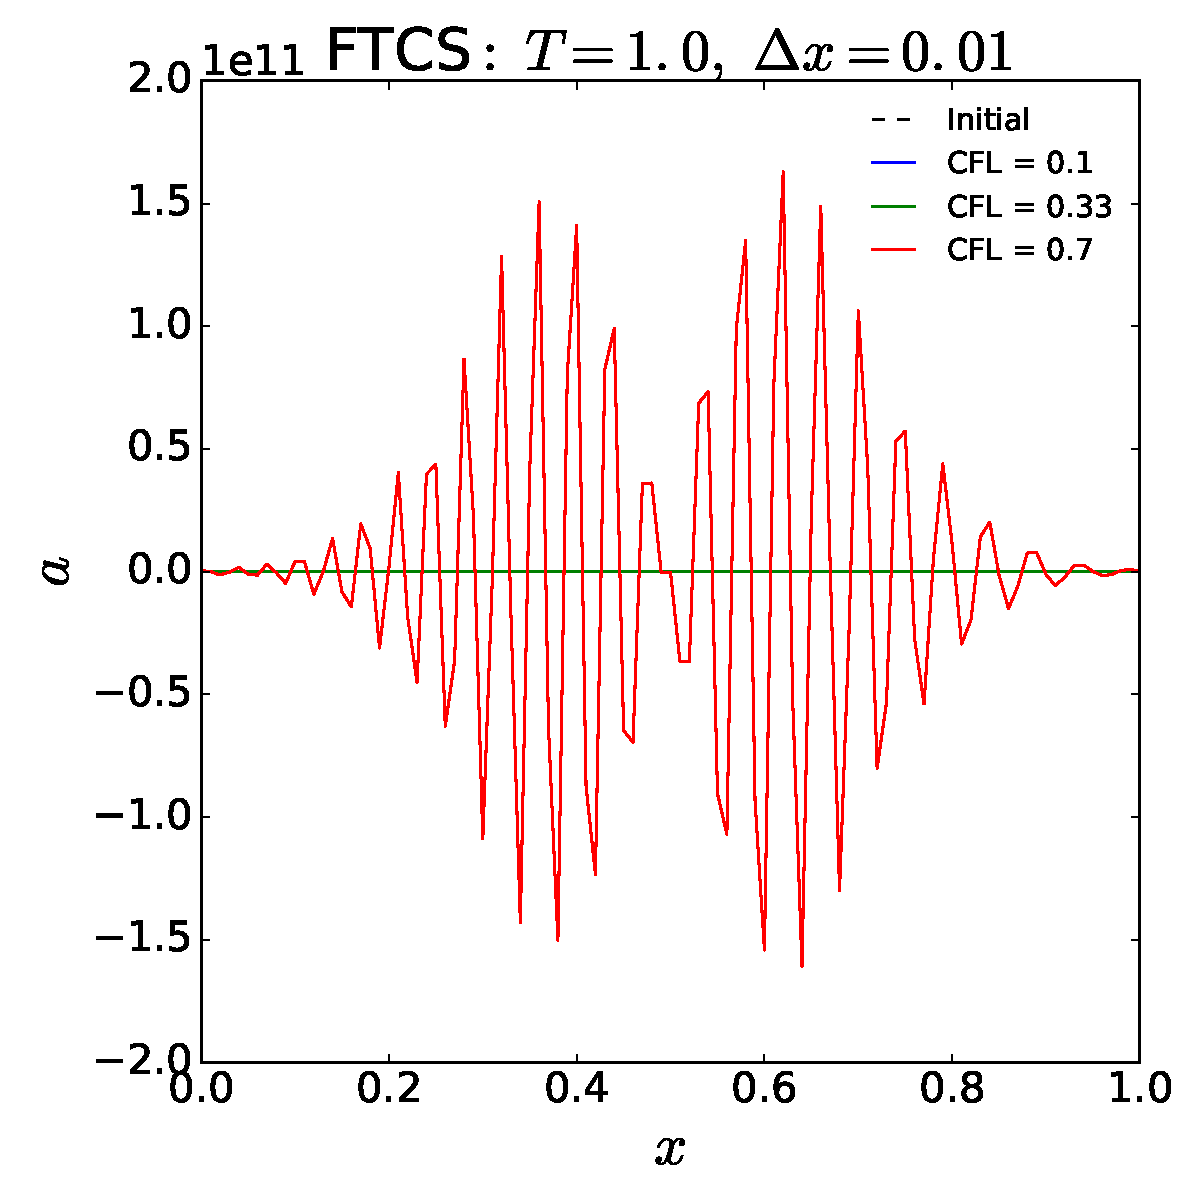
\includegraphics[width=0.45\columnwidth]{FTCS_T10_dx001.pdf}
    \caption{The system after $T=0.1$ and $T=1.0$ with resolution $\Delta x=0.01$}
    \label{fig:FTCS_dx001}
\end{figure}

\begin{figure}[h]
    \centering
    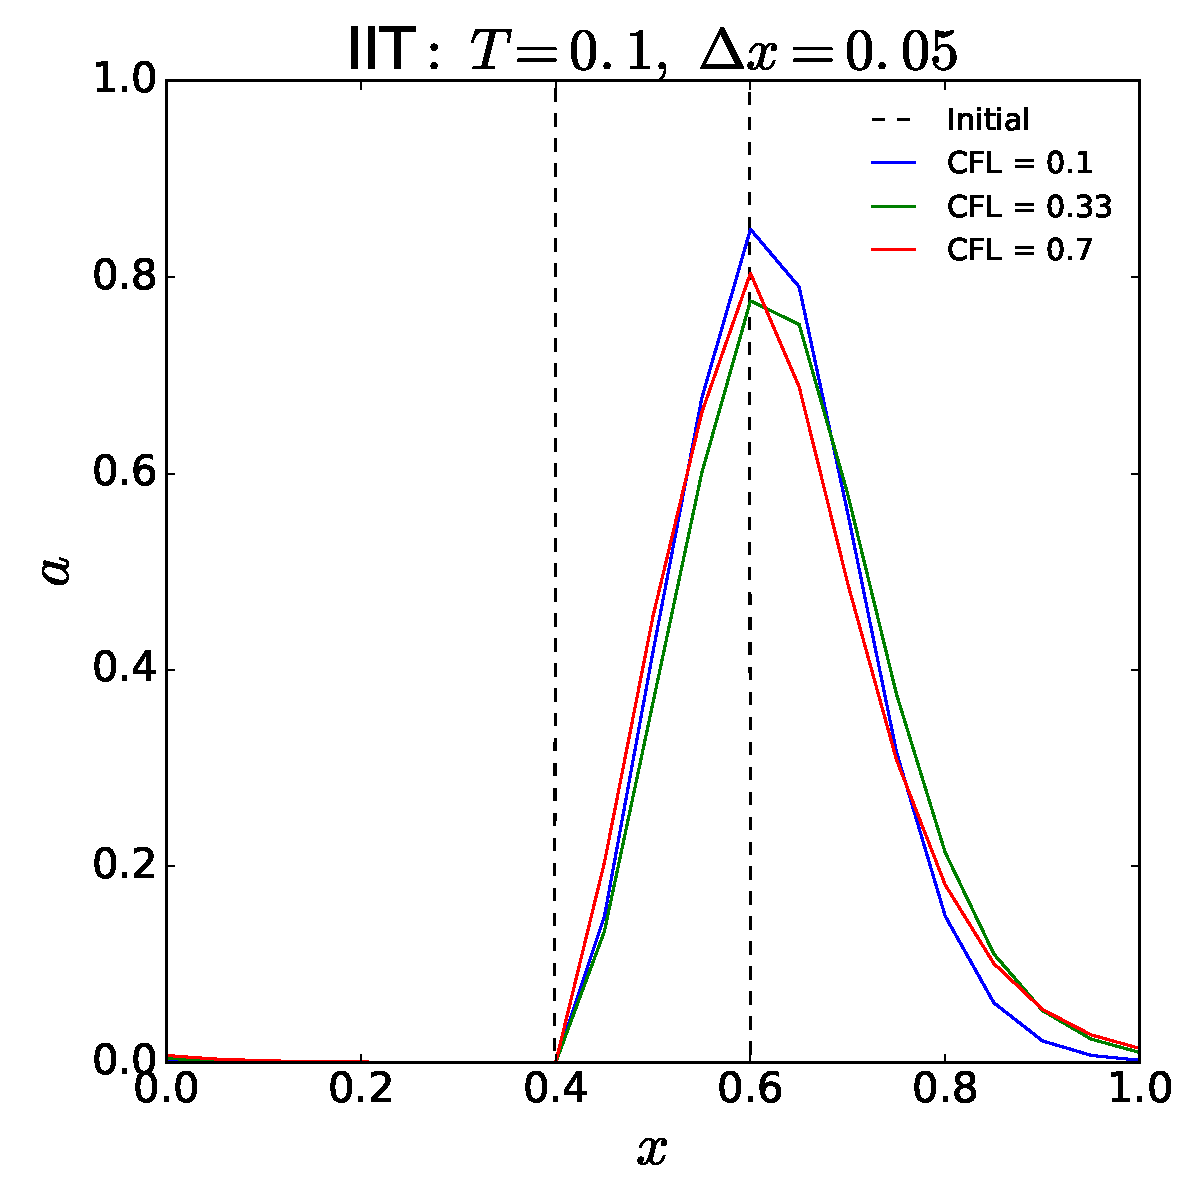
\includegraphics[width=0.45\columnwidth]{IIT_T01_dx005.pdf}
    \hspace{0.05pt}
    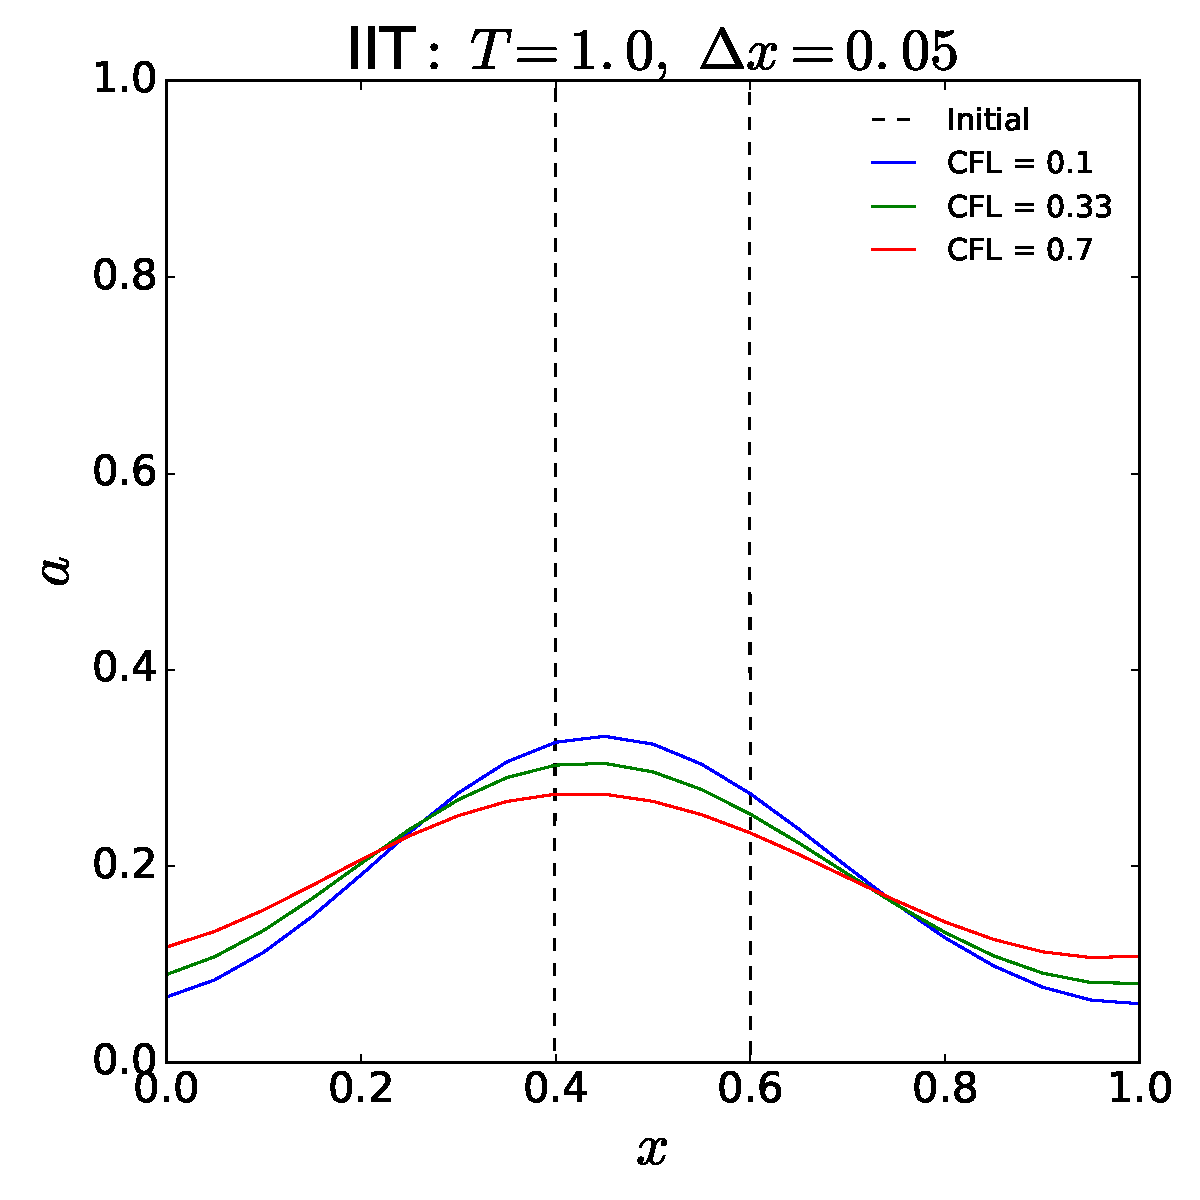
\includegraphics[width=0.45\columnwidth]{IIT_T10_dx005.pdf}
    \caption{The system after $T=0.1$ and $T=1.0$ with resolution $\Delta x=0.05$}
    \label{fig:IIT_dx005}
\end{figure}

\begin{figure}[h]
    \centering
    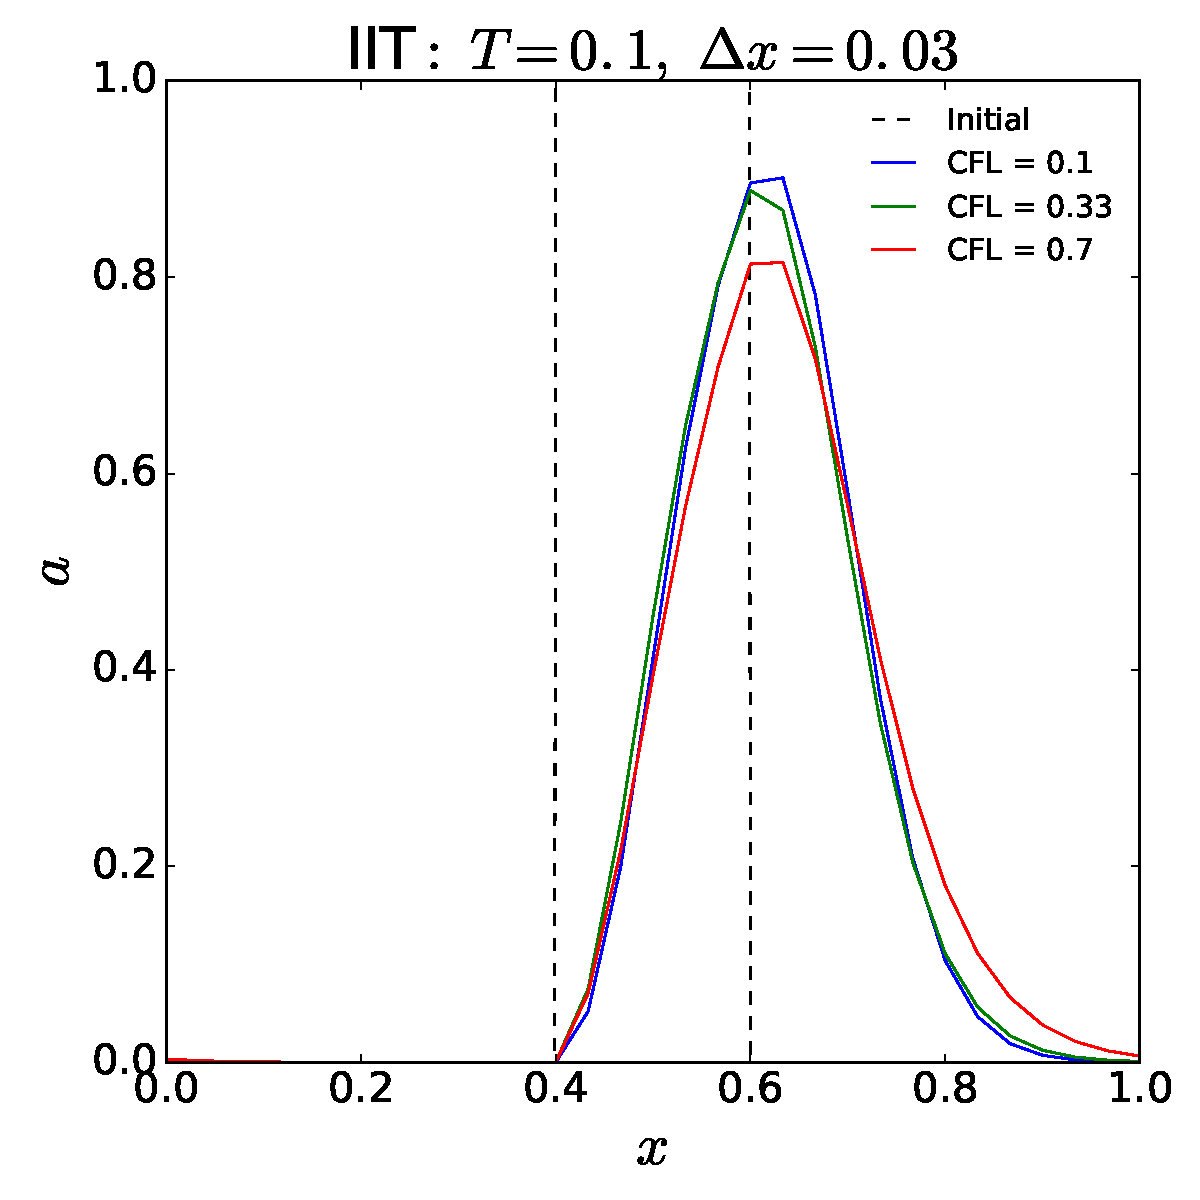
\includegraphics[width=0.45\columnwidth]{IIT_T01_dx003.pdf}
    \hspace{0.05pt}
    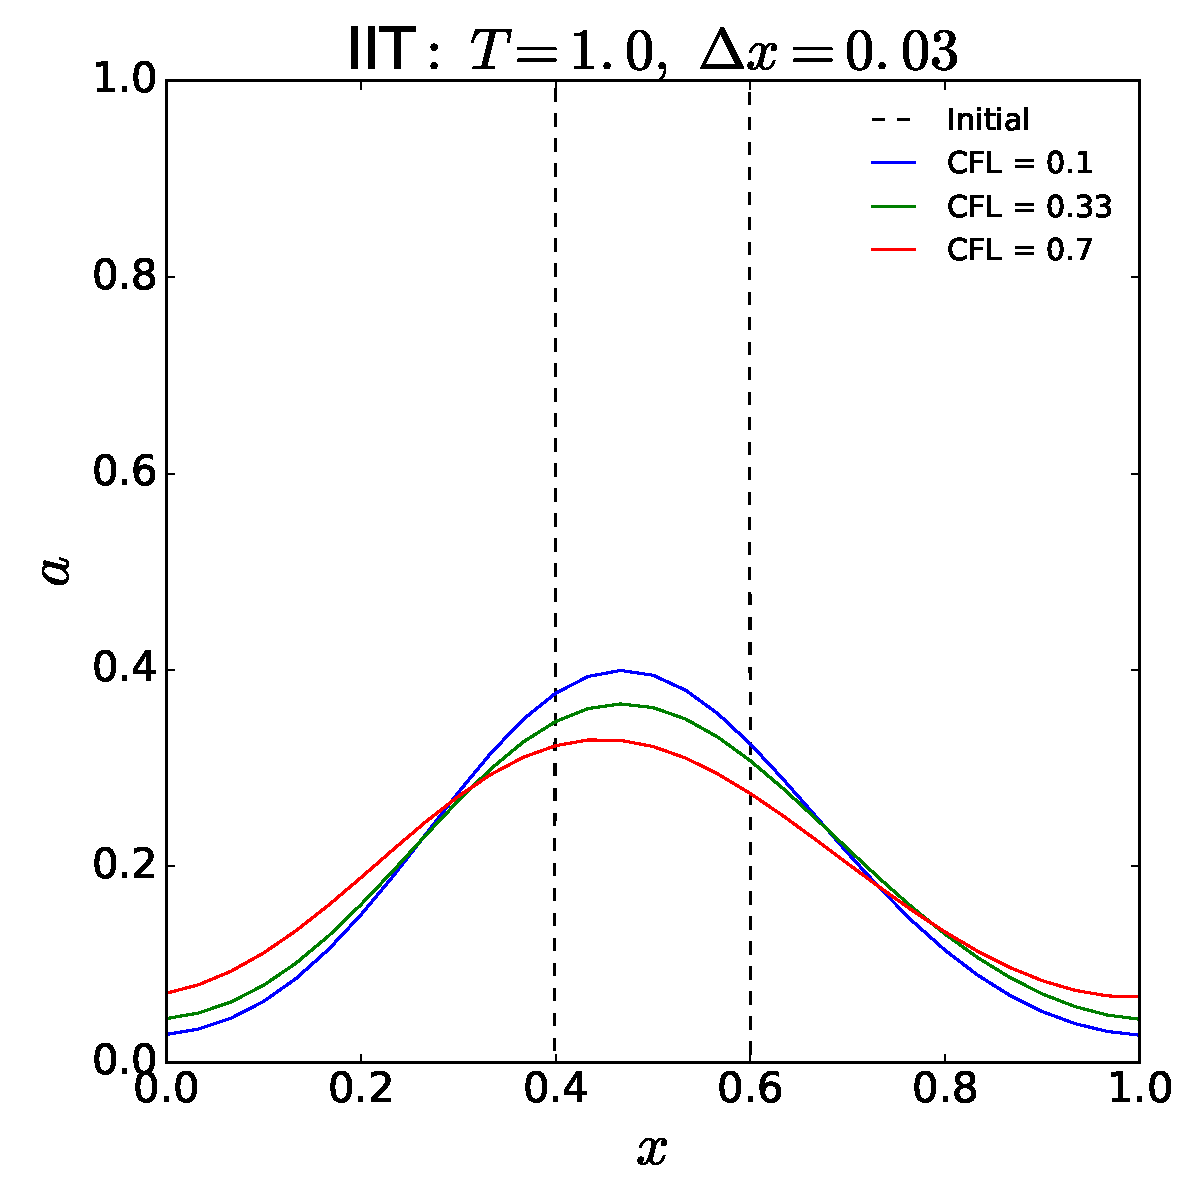
\includegraphics[width=0.45\columnwidth]{IIT_T10_dx003.pdf}
    \caption{The system after $T=0.1$ and $T=1.0$ with resolution $\Delta x=0.03$}
    \label{fig:IIT_dx003}
\end{figure}

\begin{figure}[h]
    \centering
    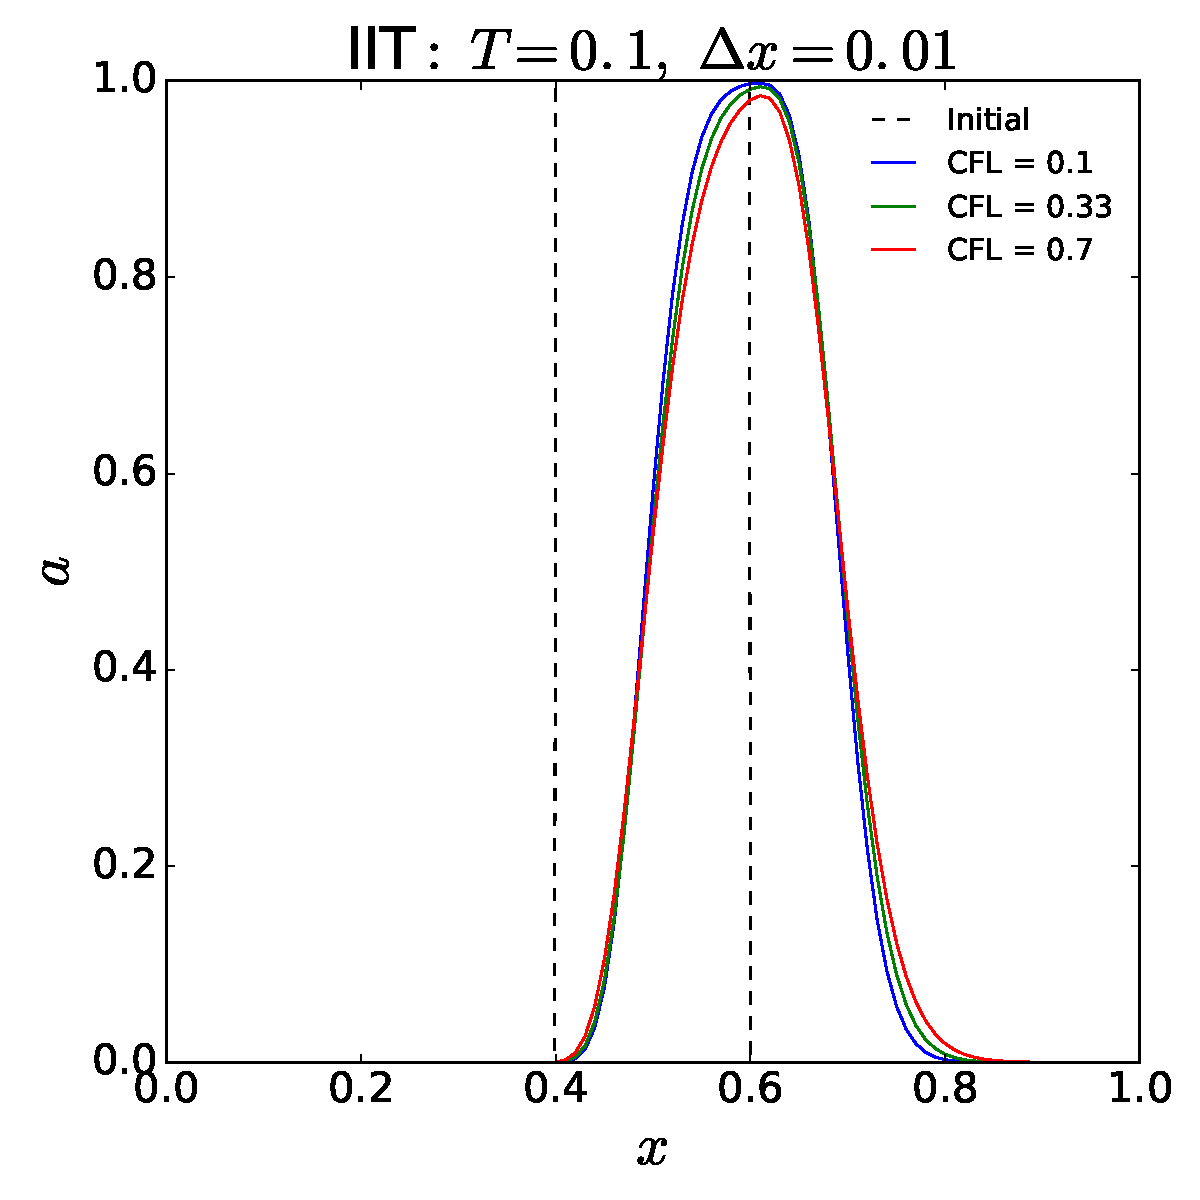
\includegraphics[width=0.45\columnwidth]{IIT_T01_dx001.pdf}
    \hspace{0.05pt}
    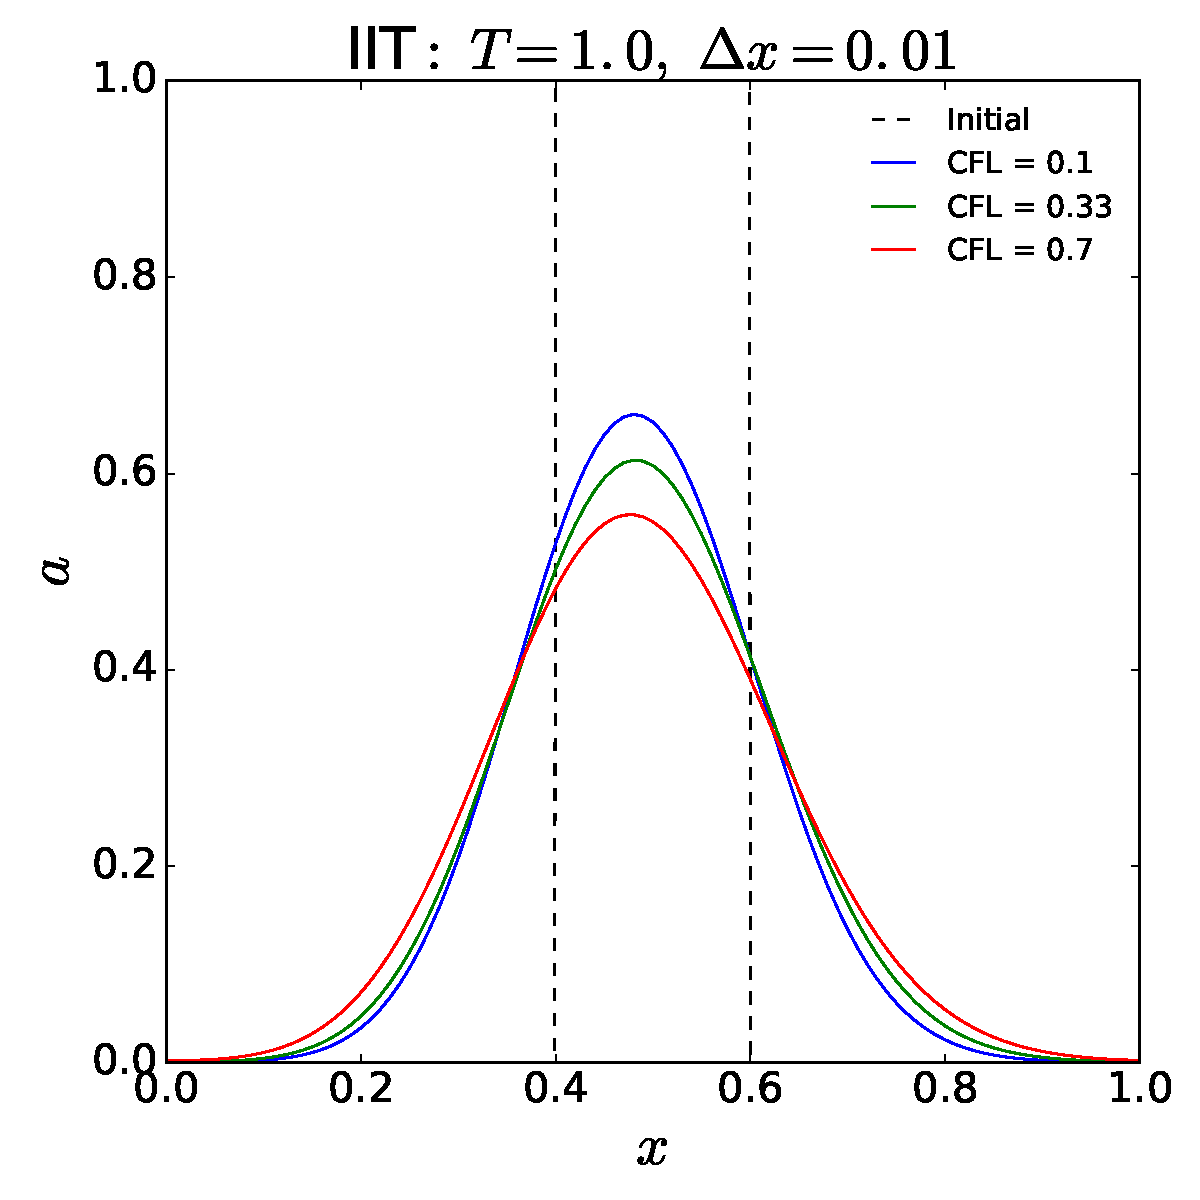
\includegraphics[width=0.45\columnwidth]{IIT_T10_dx001.pdf}
    \caption{The system after $T=0.1$ and $T=1.0$ with resolution $\Delta x=0.01$}
    \label{fig:IIT_dx001}
\end{figure}


\end{document}
    